\begin{center}
    {\LARGE \textbf{2014物理化学}} \\[2ex]
    {\large 时量180分钟 \quad 满分150分}
\end{center}

\vspace{0.5cm}
\noindent\textbf{注意事项:}
\begin{enumerate}[label=\arabic*., parsep=0pt, itemsep=0pt]
    \item 答题前,考生先将自己的姓名、学号、考场号、座位号填写在答题卡上,将条形码准确粘贴在考生信息条形码粘贴区。
    \item 考试结束后,将本试卷与答题纸一并收回。
    \item 回答各个问题时,将答案写在答题纸上,写在本试卷上无效。
\end{enumerate}

\vspace{0.5cm}
\noindent\textbf{一、选择题（30 pts.）}

\begin{enumerate}[label=\arabic*., itemsep=1.5ex]
    \item 某气体服从状态方程式$pV_\mathrm{m}=RT+bp$（$b$为大于零的常数），若该气体经等温可逆膨胀，其热力学能变化（$\Delta U$）为
    \begin{tasks}(4)
        \task $\Delta U>0$
        \task $\Delta U<0$
        \task $\Delta U=0$
        \task 不确定值
    \end{tasks}
    \item 在$300\ \mathrm{K}$时，液体$\ce{A}$和$\ce{B}$部分互溶形成$\alpha$和$\beta$两个平衡相，在$\alpha$相，$\ce{A}$的摩尔分数为$0.85$，纯$\ce{A}$的饱和蒸气压是$22\ \mathrm{kPa}$，在$\beta$相中$\ce{B}$的摩尔分数为$0.89$，将两层液相视为稀溶液，则$\ce{A}$的亨利常数为
    \begin{tasks}(4)
        \task $25.88\ \mathrm{kPa}$
        \task $200\ \mathrm{kPa}$
        \task $170\ \mathrm{kPa}$
        \task $721.2\ \mathrm{kPa}$
    \end{tasks}
    \item 一定量的理想气体从同一始态出发，分别经（1）等温压缩，（2）绝热压缩到具有相同压力的终态，以$H_1$、$H_2$分别表示两个终态的焓值，则有
    \begin{tasks}(4)
        \task $H_1>H_2$
        \task $H_1=H_2$
        \task $H_1<H_2$
        \task 不确定
    \end{tasks}
    \item 在$263\ \mathrm{K}$的过冷水凝结成$263\ \mathrm{K}$的冰，则
    \begin{tasks}(4)
        \task $\Delta S<0$
        \task $\Delta S>0$
        \task $\Delta S=0$
        \task 无法确定
    \end{tasks}
    \item 质量摩尔浓度均为$b$的不同价型电解质，设$1-3$价型电解质的离子强度为$I_1$，$2-2$价型电解质的离子强度为$I_2$，则
    \begin{tasks}(4)
        \task $I_1<I_2$
        \task $I_1=I_2$
        \task $I_1=1.5I_2$
        \task 无法比较$I_1$和$I_2$大小
    \end{tasks}
    \item 铅蓄电池工作时发生的电池反应为
    \begin{tasks}(1)
        \task $\ce{Pb(s) + SO^{2-}_{4} -> PbSO_{4}(s) + 2e^{-}}$
        \task $\ce{2PbSO_{4}(s) + 2H_{2}O(l) -> Pb(s) + PbO_{2}(s) + 2H_{2}SO_{4}(aq)}$
        \task $\ce{Pb(s) + PbO_{2}(s) + 2H_{2}SO_{4}(aq) -> 2PbSO_{4}(s) + 2H_{2}O(l)}$
        \task $\ce{PbO_{2}(s) + SO^{2-}_{4}(aq) + 4H^{+} + 2e^{-} -> PbSO_{4}(s) + 2H_{2}O(l)}$
    \end{tasks}
    \item 某放射性同位素的半衰期为$5\ \mathrm{d}$，则经$15\ \mathrm{d}$后，所剩的同位素的量是原来的
    \begin{tasks}(4)
        \task $1/3$
        \task $1/4$
        \task $1/8$
        \task $1/16$
    \end{tasks}
    \item 氯仿(1)和丙酮(2)形成非理想液体混合物，在$T$时，测得总蒸气压为$29\ 398\ \mathrm{Pa}$，蒸气中丙酮的摩尔分数$y_2=0.818$，而该温度下纯氯仿的饱和蒸气压为$29\ 571\ \mathrm{Pa}$，则在溶液中氯仿的活度$a_1$为
    \begin{tasks}(4)
        \task $0.500$
        \task $0.823$
        \task $0.181$
        \task $0.813$
    \end{tasks}
    \item 在$400\ \mathrm{K}$时，液体$\ce{A}$的蒸气压为$4\times10^4\ \mathrm{Pa}$，液体$\ce{B}$的蒸气压为$6\times10^4\ \mathrm{Pa}$，两者组成理想液体混合物，平衡时溶液中$\ce{A}$的摩尔分数为$0.6$，则气相中$\ce{B}$的摩尔分数为
    \begin{tasks}(4)
        \task $0.60$
        \task $0.50$
        \task $0.40$
        \task $0.31$
    \end{tasks}
    \item $25^\circ\mathrm{C}$时，$1\ \mathrm{mol}$理想气体等温膨胀，压力从$10p^\ominus$变到$p^\ominus$，体系吉布斯自由能变化多少？
    \begin{tasks}(4)
        \task $0.04\ \mathrm{kJ}$
        \task $-12.4\ \mathrm{kJ}$
        \task $1.24\ \mathrm{kJ}$
        \task $-5.70\ \mathrm{kJ}$
    \end{tasks}
    \item 在恒温抽空的玻璃罩中封入两杯液面相同的糖水（$\ce{A}$）和纯水（$\ce{B}$）。经历若干时间后，两杯液面的高度将是
    \begin{tasks}(4)
        \task $\ce{A}$杯高于$\ce{B}$杯
        \task $\ce{A}$杯等于$\ce{B}$杯
        \task $\ce{A}$杯低于$\ce{B}$杯
        \task 视温度而定
    \end{tasks}
    \item $1\ \mathrm{mol}$电子电荷量与下列哪一个值相同？
    \begin{tasks}(4)
        \task $1$安培·秒
        \task $1$库仑
        \task $1$法拉第
        \task $1$居里
    \end{tasks}
    \item 为马拉松运动员沿途准备的饮料应该是哪一种？
    \begin{tasks}(2)
        \task 高脂肪、高蛋白、高能量饮料
        \task $20\%$葡萄糖水
        \task 含适量维生素的等渗饮料
        \task 含兴奋剂的饮料
    \end{tasks}
    \item 已知$25^\circ\mathrm{C}$时，电极反应$\displaystyle \frac{1}{2}\ce{O_{2} + H_{2}O + 2e^{-} -> 2OH^{-}}$的标准电极电势为$\varphi^\ominus_1=0.401\ \mathrm{V}$，则$25^\circ\mathrm{C}$时，电极反应$\displaystyle \frac{1}{2}\ce{O_{2} + 2H^{+} + 2e^{-} -> H_{2}O}$的标准电极电势$\varphi^\ominus_2$为（设$K_\mathrm{w}=1\times10^{-14}$）
    \begin{tasks}(4)
        \task $-0.427\ \mathrm{V}$
        \task $0.401\ \mathrm{V}$
        \task $0.828\ \mathrm{V}$
        \task $1.229\ \mathrm{V}$
    \end{tasks}
    \item $p^\ominus$和$298\ \mathrm{K}$下，把$\ce{Pb}$和$\ce{Cu(Ac)_{2}}$溶液发生的反应安排为电池，当获得可逆电功
    
    为$91.84\ \mathrm{kJ}$时，电池同时吸热$213.6\ \mathrm{kJ}$，因此该过程有
    \begin{tasks}(2)
        \task $\Delta_\mathrm{r}U>0$，$\Delta_\mathrm{r}S>0$
        \task $\Delta_\mathrm{r}U<0$，$\Delta_\mathrm{r}S>0$
        \task $\Delta_\mathrm{r}U>0$，$\Delta_\mathrm{r}S<0$
        \task $\Delta_\mathrm{r}U<0$，$\Delta_\mathrm{r}S<0$
    \end{tasks}
\end{enumerate}

\vspace{0.5cm}
\noindent\textbf{二、计算题（20 pts.）}

甲烷的蒸气压与热力学温度$T$如下式所示：
\[
\lg(p/\mathrm{Pa}) = 8.96 - 445/(T/\mathrm{K})
\]
甲烷的正常沸点为$112\ \mathrm{K}$。
(1) 在$p^\ominus$、$112\ \mathrm{K}$下，$1\ \mathrm{mol}\ \ce{CH_{4}(l)}$等温可逆变化为$1\ \mathrm{mol}\ \ce{CH_{4}(g)}$；
(2) $1\ \mathrm{mol}\ \ce{CH_{4}(l,p^\ominus,112\ \mathrm{K})}$在真空条件下变化为$1\ \mathrm{mol}\ \ce{CH_{4}(g,p^\ominus,112\ \mathrm{K})}$。
试分别计算(1)和(2)过程的$Q$、$W$、$\Delta S_\text{体}$、$\Delta S_\text{环}$和$\Delta S_\text{总}$。

\vspace{0.5cm}
\noindent\textbf{三、计算题（15 pts.）}

在$101\ 325\ \mathrm{Pa}$下，$293\ \mathrm{K}$和$313\ \mathrm{K}$时，$\ce{CO_{2}}$气体在$1\ \mathrm{kg}$水中分别可溶解$1.7\times10^{-3}\ \mathrm{kg}$和$1\times10^{-3}\ \mathrm{kg}$，如果用只能承受$202\ 650\ \mathrm{Pa}$的瓶子充装含$\ce{CO_{2}}$的饮料，则在$293\ \mathrm{K}$时，$\ce{CO_{2}}$的最大压力应为多少时才能保证这种瓶装饮料可以在$313\ \mathrm{K}$条件下安全存放？设溶质服从亨利定律，$\ce{CO_{2}}$的摩尔质量为$0.044\ \mathrm{kg\cdot mol^{-1}}$。

\vspace{0.5cm}
\noindent\textbf{四、计算题（20 pts.）}

下图是$p^\ominus$下$\ce{SiO_{2}-Al_{2}O_{3}}$体系在高温区间的相图，本相图在耐火材料工业上具有重要意义，在高温下，$\ce{SiO_{2}}$有白硅石和鳞石英两种变体，$AB$是这两种变体的转晶线，$AB$线之上为白硅石，之下为鳞石英。（莫莱石的组成为$\ce{2Al_{2}O_{3}\cdot 3SiO_{2}}$）

\begin{figure}[htbp]
    \centering
    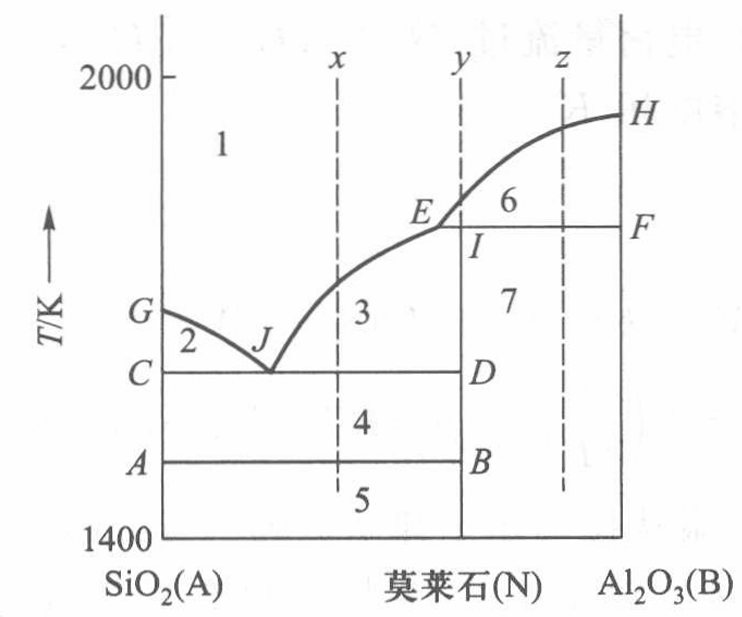
\includegraphics[width=0.52\textwidth]{./Figure/P_2014_4}

\end{figure}

\begin{enumerate}[label=(\arabic*), itemsep=1ex]
    \item 指出各相区的相组成；
    \item 指出$GJ$,$JE$,$JH$,$CD$,$EF$相线和各相区的自由度；
    \item 图中三条水平线分别代表哪些相平衡共存；
    \item 画出从$x$,$y$,$z$点冷却的步冷曲线。
\end{enumerate}

\vspace{0.5cm}
\noindent\textbf{五、计算题(15 pts.)}

$\ce{Ag2CO3(s)}$分解反应方程为$\ce{Ag2CO3(s) -> Ag2O(s) + CO2(g)}$,设气相为理想气体,$298\ \mathrm{K}$时各物质的$\Delta_\mathrm{f}H_\mathrm{m}^\ominus$、$S_\mathrm{m}^\ominus$如下：

\begin{center}
\begin{tabular}{lcc}
 & $\Delta_\mathrm{f}H_\mathrm{m}^\ominus/(\mathrm{kJ\cdot mol^{-1}})$ & $S_\mathrm{m}^\ominus/(\mathrm{J\cdot K^{-1}\cdot mol^{-1}})$ \\
$\ce{Ag2CO3(s)}$ & $-506.14$ & $167.36$ \\
$\ce{Ag2O(s)}$ & $-30.57$ & $121.71$ \\
$\ce{CO2(g)}$ & $-393.15$ & $213.64$ \\
\end{tabular}
\end{center}

\begin{enumerate}[label=(\arabic*), itemsep=1ex]
    \item 求$298\ \mathrm{K}$,$101\ 352\ \mathrm{Pa}$下,$1\mathrm{mol}\ \ce{Ag2CO3(s)}$完全分解时吸收的热量；
    \item 求$298\ \mathrm{K}$下,$\ce{Ag2CO3(s)}$的分解压力；
    \item 假设反应焓变与温度无关,求$383\ \mathrm{K}$下$\ce{Ag2CO3}$分解时的平衡压力；
    \item 求体系组分数与自由度。
\end{enumerate}

\vspace{0.5cm}
\noindent\textbf{六、计算题(15 pts.)}

$\ce{ClCOOCCl3}$热分解反应:$\ce{ClCOOCCl3(g) -> 2COCl2(g)}$是一级反应,一定量$\ce{ClCOOCCl3}$迅速引入一个$553\ \mathrm{K}$的容器中,经$454\ \mathrm{s}$,测得压力为$2.475\ \mathrm{kPa}$,经过极长时间后压力为$4.008\ \mathrm{kPa}$,此实验在$578\ \mathrm{K}$时重复一次,经过$320\ \mathrm{s}$后,测得压力为$2.838\ \mathrm{kPa}$,求此分解反应活化能$E_\mathrm{a}$。

\vspace{0.5cm}
\noindent\textbf{七、计算题(15 pts.)}

反应$\ce{Zn(s) + CuSO4(a=1) -> Cu(s) + ZnSO4(a=1)}$在电池中进行,$15^\circ\mathrm{C}$时,$\varphi(\ce{Cu^{2+} | Cu})=0.340\ \mathrm{V}$,$\varphi(\ce{Zn^{2+} | Zn})=-0.76\ \mathrm{V}$,电池的温度系数$(\partial E/\partial T)_p=-4.29\times10^{-4}\ \mathrm{V\cdot K^{-1}}$,
\begin{enumerate}[label=(\arabic*), itemsep=1ex]
    \item 写出电池表示式,电极反应式；
    \item 计算$15^\circ\mathrm{C}$时电池的电动式$E$；
    \item 求电池反应的$\Delta_\mathrm{r}G_\mathrm{m}^\ominus$,$\Delta_\mathrm{r}S_\mathrm{m}^\ominus$,$\Delta_\mathrm{r}H_\mathrm{m}^\ominus$和$Q_\mathrm{r}$。
\end{enumerate}

\vspace{0.5cm}
\noindent\textbf{八、计算题(20 pts.)}

电池$\ce{Cu(s) | CuAc2(0.1\ mol\cdot kg^{-1}) | AgAc(s),Ag(s)}$在$298\ \mathrm{K}$时,电动势$E=0.372\ \mathrm{V}$,当温度升至$308\ \mathrm{K}$时,$E=0.374\ \mathrm{V}$,已知$298\ \mathrm{K}$时$\varphi(\ce{Ag+ | Ag})=0.800\ \mathrm{V}$,$\varphi(\ce{Cu^{2+} | Cu})=0.340\ \mathrm{V}$,各离子活度系数为$1$,
\begin{enumerate}[label=(\arabic*), itemsep=1ex]
    \item 写出电极的反应和电池反应；
    \item $298\ \mathrm{K}$时,当电池有$2F$电荷量流过,这时$\Delta_\mathrm{r}G_\mathrm{m}$,$\Delta_\mathrm{r}H_\mathrm{m}$,$\Delta_\mathrm{r}S_\mathrm{m}$为多少?
    \item 计算醋酸银$\ce{AgAc}$的溶度积$K_{\mathrm{sp}}$。
\end{enumerate}